\section{Schaffer Function N.4}
  The \emph{Schaffer Function N.4} is a mathematical function used as a 
  performance test problem for optimization algorithms.
  It is particularly suited for testing algorithms that need to optimize 
  complex, non-linear problems with many local minima.

  \begin{definition}[Schaffer Function N.4]
    Schaffer Function N.4 is defined as follows:

    For \(x \in \mathbb{R}^2\), the function is given by:

    \[
      f(x) = 0.5 
        + \frac{
            \cos^2\left(\sin\left[\left|x^2 - y^2\right|\right]\right) - 0.5
          }{
            \left[1 + 0.001\left(x^2 + y^2\right)\right]^2
          }
    \]

    Where:
    \begin{itemize}
      \item \(x\) and \(y\) are decision variables.
      \item The function has four global minima of \(0.292579\), located at 
        \(0,\, \pm 1.25313\) and \(\pm 1.25313,\, 0\).
    \end{itemize}
  \end{definition}

  The characteristic feature of Schaffer N.4 is its landscape with several local minima and four global minima.
  This structure poses a significant challenge to optimization algorithms, especially those prone to being trapped in local minima.


  Figure \ref{fig:app:test:schaffer_4} provides a visualization of the Schaffer 
  Function N.4.
  The contour and surface plots show the function's topology, with the red dots 
  indicating the locations of the global minima.
  The close-up contour and surface plots offer a detailed view of the global 
  minima and their immediate surroundings, highlighting the intricacy of the 
  function's landscape.


  \begin{figure}[ht!]
    \centering
    \begin{subfigure}[b]{0.45\textwidth}
      \centering
      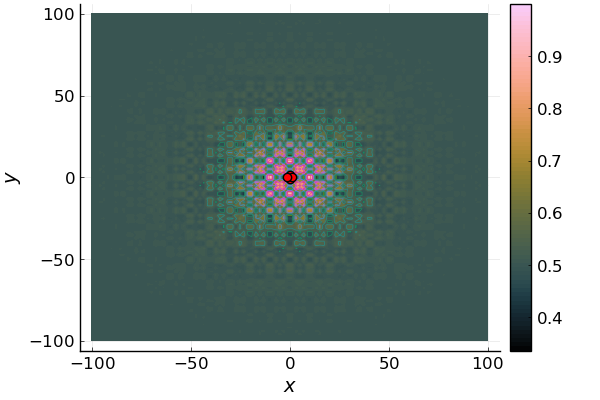
\includegraphics[width=\textwidth]
        {img/test_functions/schaffer_4_contour.png}
      \caption{Contour plot of the Schaffer Function N.4}
    \end{subfigure}
    \hfill
    \begin{subfigure}[b]{0.45\textwidth}
      \centering
      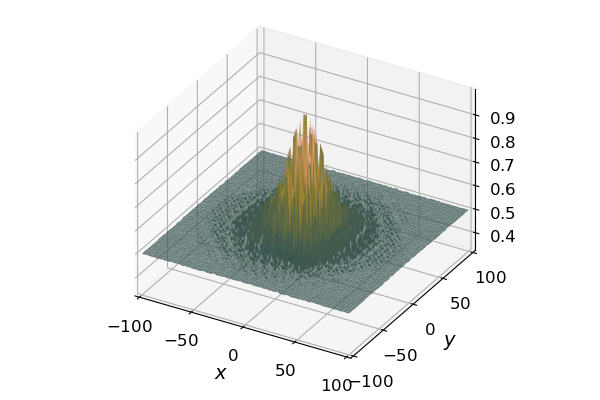
\includegraphics[width=\textwidth]
        {img/test_functions/schaffer_4_surface.png}
      \caption{Surface plot of the Schaffer Function N.4}
    \end{subfigure}
    \begin{subfigure}[b]{0.45\textwidth}
      \centering
      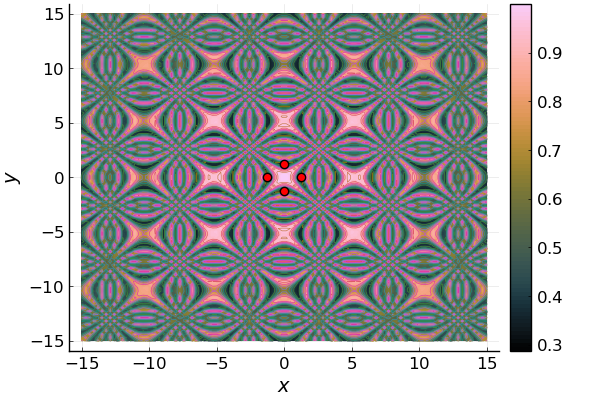
\includegraphics[width=\textwidth]
        {img/test_functions/schaffer_4_closeup_contour.png}
      \caption{
        Close-up contour plot of the Schaffer Function N.4 in the vicinity of
        the global minimum.
      }
    \end{subfigure}
    \hfill
    \begin{subfigure}[b]{0.45\textwidth}
      \centering
      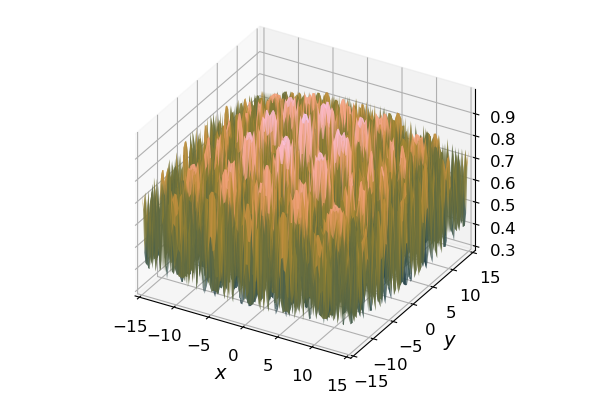
\includegraphics[width=\textwidth]
        {img/test_functions/schaffer_4_closeup_surface.png}
      \caption{
        Close-up surface plot of the Schaffer Function N.4 in the vicinity of
        the global minimum.
      }
    \end{subfigure}
    \caption{
      Visualization of the Schaffer Function N.4.
      The contour and surface plots illustrate the function's topology, with the
      global minimum denoted by a red dot.
      The close-up contour and surface plots provide a more precise view of the 
      global minimum and the immediate surroundings.
    }
    \label{fig:app:test:schaffer_4}
  \end{figure}
